
%% bare_conf.tex
%% V1.3
%% 2007/01/11
%% by Michael Shell
%% See:
%% http://www.michaelshell.org/
%% for current contact information.
%%
%% This is a skeleton file demonstrating the use of IEEEtran.cls
%% (requires IEEEtran.cls version 1.7 or later) with an IEEE conference paper.
%%
%% Support sites:
%% http://www.michaelshell.org/tex/ieeetran/
%% http://www.ctan.org/tex-archive/macros/latex/contrib/IEEEtran/
%% and
%% http://www.ieee.org/

%%*************************************************************************
%% Legal Notice:
%% This code is offered as-is without any warranty either expressed or
%% implied; without even the implied warranty of MERCHANTABILITY or
%% FITNESS FOR A PARTICULAR PURPOSE! 
%% User assumes all risk.
%% In no event shall IEEE or any contributor to this code be liable for
%% any damages or losses, including, but not limited to, incidental,
%% consequential, or any other damages, resulting from the use or misuse
%% of any information contained here.
%%
%% All comments are the opinions of their respective authors and are not
%% necessarily endorsed by the IEEE.
%%
%% This work is distributed under the LaTeX Project Public License (LPPL)
%% ( http://www.latex-project.org/ ) version 1.3, and may be freely used,
%% distributed and modified. A copy of the LPPL, version 1.3, is included
%% in the base LaTeX documentation of all distributions of LaTeX released
%% 2003/12/01 or later.
%% Retain all contribution notices and credits.
%% ** Modified files should be clearly indicated as such, including  **
%% ** renaming them and changing author support contact information. **
%%
%% File list of work: IEEEtran.cls, IEEEtran_HOWTO.pdf, bare_adv.tex,
%%                    bare_conf.tex, bare_jrnl.tex, bare_jrnl_compsoc.tex
%%*************************************************************************

% *** Authors should verify (and, if needed, correct) their LaTeX system  ***
% *** with the testflow diagnostic prior to trusting their LaTeX platform ***
% *** with production work. IEEE's font choices can trigger bugs that do  ***
% *** not appear when using other class files.                            ***
% The testflow support page is at:
% http://www.michaelshell.org/tex/testflow/



% Note that the a4paper option is mainly intended so that authors in
% countries using A4 can easily print to A4 and see how their papers will
% look in print - the typesetting of the document will not typically be
% affected with changes in paper size (but the bottom and side margins will).
% Use the testflow package mentioned above to verify correct handling of
% both paper sizes by the user's LaTeX system.
%
% Also note that the "draftcls" or "draftclsnofoot", not "draft", option
% should be used if it is desired that the figures are to be displayed in
% draft mode.
%
\documentclass[conference]{IEEEtran}
% Add the compsoc option for Computer Society conferences.
%
% If IEEEtran.cls has not been installed into the LaTeX system files,
% manually specify the path to it like:
% \documentclass[conference]{../sty/IEEEtran}





% Some very useful LaTeX packages include:
% (uncomment the ones you want to load)


% *** MISC UTILITY PACKAGES ***
%
%\usepackage{ifpdf}
% Heiko Oberdiek's ifpdf.sty is very useful if you need conditional
% compilation based on whether the output is pdf or dvi.
% usage:
% \ifpdf
%   % pdf code
% \else
%   % dvi code
% \fi
% The latest version of ifpdf.sty can be obtained from:
% http://www.ctan.org/tex-archive/macros/latex/contrib/oberdiek/
% Also, note that IEEEtran.cls V1.7 and later provides a builtin
% \ifCLASSINFOpdf conditional that works the same way.
% When switching from latex to pdflatex and vice-versa, the compiler may
% have to be run twice to clear warning/error messages.






% *** CITATION PACKAGES ***
%
%\usepackage{cite}
% cite.sty was written by Donald Arseneau
% V1.6 and later of IEEEtran pre-defines the format of the cite.sty package
% \cite{} output to follow that of IEEE. Loading the cite package will
% result in citation numbers being automatically sorted and properly
% "compressed/ranged". e.g., [1], [9], [2], [7], [5], [6] without using
% cite.sty will become [1], [2], [5]--[7], [9] using cite.sty. cite.sty's
% \cite will automatically add leading space, if needed. Use cite.sty's
% noadjust option (cite.sty V3.8 and later) if you want to turn this off.
% cite.sty is already installed on most LaTeX systems. Be sure and use
% version 4.0 (2003-05-27) and later if using hyperref.sty. cite.sty does
% not currently provide for hyperlinked citations.
% The latest version can be obtained at:
% http://www.ctan.org/tex-archive/macros/latex/contrib/cite/
% The documentation is contained in the cite.sty file itself.





\usepackage[pdftex]{graphicx}
\graphicspath{{images/}}
% *** GRAPHICS RELATED PACKAGES ***
%
\ifCLASSINFOpdf
  % \usepackage[pdftex]{graphicx}
  % declare the path(s) where your graphic files are
  % \graphicspath{{../pdf/}{../jpeg/}}
  % and their extensions so you won't have to specify these with
  % every instance of \includegraphics
  % \DeclareGraphicsExtensions{.pdf,.jpeg,.png}
\else
  % or other class option (dvipsone, dvipdf, if not using dvips). graphicx
  % will default to the driver specified in the system graphics.cfg if no
  % driver is specified.
  % \usepackage[dvips]{graphicx}
  % declare the path(s) where your graphic files are
  % \graphicspath{{../eps/}}
  % and their extensions so you won't have to specify these with
  % every instance of \includegraphics
  % \DeclareGraphicsExtensions{.eps}
\fi
% graphicx was written by David Carlisle and Sebastian Rahtz. It is
% required if you want graphics, photos, etc. graphicx.sty is already
% installed on most LaTeX systems. The latest version and documentation can
% be obtained at: 
% http://www.ctan.org/tex-archive/macros/latex/required/graphics/
% Another good source of documentation is "Using Imported Graphics in
% LaTeX2e" by Keith Reckdahl which can be found as epslatex.ps or
% epslatex.pdf at: http://www.ctan.org/tex-archive/info/
%
% latex, and pdflatex in dvi mode, support graphics in encapsulated
% postscript (.eps) format. pdflatex in pdf mode supports graphics
% in .pdf, .jpeg, .png and .mps (metapost) formats. Users should ensure
% that all non-photo figures use a vector format (.eps, .pdf, .mps) and
% not a bitmapped formats (.jpeg, .png). IEEE frowns on bitmapped formats
% which can result in "jaggedy"/blurry rendering of lines and letters as
% well as large increases in file sizes.
%
% You can find documentation about the pdfTeX application at:
% http://www.tug.org/applications/pdftex





% *** MATH PACKAGES ***
%
\usepackage[cmex10]{amsmath}
% A popular package from the American Mathematical Society that provides
% many useful and powerful commands for dealing with mathematics. If using
% it, be sure to load this package with the cmex10 option to ensure that
% only type 1 fonts will utilized at all point sizes. Without this option,
% it is possible that some math symbols, particularly those within
% footnotes, will be rendered in bitmap form which will result in a
% document that can not be IEEE Xplore compliant!
%
% Also, note that the amsmath package sets \interdisplaylinepenalty to 10000
% thus preventing page breaks from occurring within multiline equations. Use:
%\interdisplaylinepenalty=2500
% after loading amsmath to restore such page breaks as IEEEtran.cls normally
% does. amsmath.sty is already installed on most LaTeX systems. The latest
% version and documentation can be obtained at:
% http://www.ctan.org/tex-archive/macros/latex/required/amslatex/math/





% *** SPECIALIZED LIST PACKAGES ***
%
%\usepackage{algorithmic}
% algorithmic.sty was written by Peter Williams and Rogerio Brito.
% This package provides an algorithmic environment fo describing algorithms.
% You can use the algorithmic environment in-text or within a figure
% environment to provide for a floating algorithm. Do NOT use the algorithm
% floating environment provided by algorithm.sty (by the same authors) or
% algorithm2e.sty (by Christophe Fiorio) as IEEE does not use dedicated
% algorithm float types and packages that provide these will not provide
% correct IEEE style captions. The latest version and documentation of
% algorithmic.sty can be obtained at:
% http://www.ctan.org/tex-archive/macros/latex/contrib/algorithms/
% There is also a support site at:
% http://algorithms.berlios.de/index.html
% Also of interest may be the (relatively newer and more customizable)
% algorithmicx.sty package by Szasz Janos:
% http://www.ctan.org/tex-archive/macros/latex/contrib/algorithmicx/




% *** ALIGNMENT PACKAGES ***
%
%\usepackage{array}
% Frank Mittelbach's and David Carlisle's array.sty patches and improves
% the standard LaTeX2e array and tabular environments to provide better
% appearance and additional user controls. As the default LaTeX2e table
% generation code is lacking to the point of almost being broken with
% respect to the quality of the end results, all users are strongly
% advised to use an enhanced (at the very least that provided by array.sty)
% set of table tools. array.sty is already installed on most systems. The
% latest version and documentation can be obtained at:
% http://www.ctan.org/tex-archive/macros/latex/required/tools/


%\usepackage{mdwmath}
%\usepackage{mdwtab}
% Also highly recommended is Mark Wooding's extremely powerful MDW tools,
% especially mdwmath.sty and mdwtab.sty which are used to format equations
% and tables, respectively. The MDWtools set is already installed on most
% LaTeX systems. The lastest version and documentation is available at:
% http://www.ctan.org/tex-archive/macros/latex/contrib/mdwtools/


% IEEEtran contains the IEEEeqnarray family of commands that can be used to
% generate multiline equations as well as matrices, tables, etc., of high
% quality.


%\usepackage{eqparbox}
% Also of notable interest is Scott Pakin's eqparbox package for creating
% (automatically sized) equal width boxes - aka "natural width parboxes".
% Available at:
% http://www.ctan.org/tex-archive/macros/latex/contrib/eqparbox/





% *** SUBFIGURE PACKAGES ***
%\usepackage[tight,footnotesize]{subfigure}
% subfigure.sty was written by Steven Douglas Cochran. This package makes it
% easy to put subfigures in your figures. e.g., "Figure 1a and 1b". For IEEE
% work, it is a good idea to load it with the tight package option to reduce
% the amount of white space around the subfigures. subfigure.sty is already
% installed on most LaTeX systems. The latest version and documentation can
% be obtained at:
% http://www.ctan.org/tex-archive/obsolete/macros/latex/contrib/subfigure/
% subfigure.sty has been superceeded by subfig.sty.



%\usepackage[caption=false]{caption}
%\usepackage[font=footnotesize]{subfig}
% subfig.sty, also written by Steven Douglas Cochran, is the modern
% replacement for subfigure.sty. However, subfig.sty requires and
% automatically loads Axel Sommerfeldt's caption.sty which will override
% IEEEtran.cls handling of captions and this will result in nonIEEE style
% figure/table captions. To prevent this problem, be sure and preload
% caption.sty with its "caption=false" package option. This is will preserve
% IEEEtran.cls handing of captions. Version 1.3 (2005/06/28) and later 
% (recommended due to many improvements over 1.2) of subfig.sty supports
% the caption=false option directly:
%\usepackage[caption=false,font=footnotesize]{subfig}
%
% The latest version and documentation can be obtained at:
% http://www.ctan.org/tex-archive/macros/latex/contrib/subfig/
% The latest version and documentation of caption.sty can be obtained at:
% http://www.ctan.org/tex-archive/macros/latex/contrib/caption/




% *** FLOAT PACKAGES ***
%
%\usepackage{fixltx2e}
% fixltx2e, the successor to the earlier fix2col.sty, was written by
% Frank Mittelbach and David Carlisle. This package corrects a few problems
% in the LaTeX2e kernel, the most notable of which is that in current
% LaTeX2e releases, the ordering of single and double column floats is not
% guaranteed to be preserved. Thus, an unpatched LaTeX2e can allow a
% single column figure to be placed prior to an earlier double column
% figure. The latest version and documentation can be found at:
% http://www.ctan.org/tex-archive/macros/latex/base/



%\usepackage{stfloats}
% stfloats.sty was written by Sigitas Tolusis. This package gives LaTeX2e
% the ability to do double column floats at the bottom of the page as well
% as the top. (e.g., "\begin{figure*}[!b]" is not normally possible in
% LaTeX2e). It also provides a command:
%\fnbelowfloat
% to enable the placement of footnotes below bottom floats (the standard
% LaTeX2e kernel puts them above bottom floats). This is an invasive package
% which rewrites many portions of the LaTeX2e float routines. It may not work
% with other packages that modify the LaTeX2e float routines. The latest
% version and documentation can be obtained at:
% http://www.ctan.org/tex-archive/macros/latex/contrib/sttools/
% Documentation is contained in the stfloats.sty comments as well as in the
% presfull.pdf file. Do not use the stfloats baselinefloat ability as IEEE
% does not allow \baselineskip to stretch. Authors submitting work to the
% IEEE should note that IEEE rarely uses double column equations and
% that authors should try to avoid such use. Do not be tempted to use the
% cuted.sty or midfloat.sty packages (also by Sigitas Tolusis) as IEEE does
% not format its papers in such ways.





% *** PDF, URL AND HYPERLINK PACKAGES ***
%
%\usepackage{url}
% url.sty was written by Donald Arseneau. It provides better support for
% handling and breaking URLs. url.sty is already installed on most LaTeX
% systems. The latest version can be obtained at:
% http://www.ctan.org/tex-archive/macros/latex/contrib/misc/
% Read the url.sty source comments for usage information. Basically,
% \url{my_url_here}.





% *** Do not adjust lengths that control margins, column widths, etc. ***
% *** Do not use packages that alter fonts (such as pslatex).         ***
% There should be no need to do such things with IEEEtran.cls V1.6 and later.
% (Unless specifically asked to do so by the journal or conference you plan
% to submit to, of course. )


% correct bad hyphenation here
\hyphenation{op-tical net-works semi-conduc-tor}


\begin{document}
%
% paper title
% can use linebreaks \\ within to get better formatting as desired
\title{Framework of Marketing or Newsletter Sender Reputation System (FMNSRS)}


% author names and affiliations
% use a multiple column layout for up to three different
% affiliations


\author{\IEEEauthorblockN{Akkarach  Kawbunjun\\ and Woraphon Lilakiatsakun}
\IEEEauthorblockA{Faculty of Information Science and Technology\\
Mahanakorn University of Technology\\
Bangkok, Thailand\\
Email: akkarach@cri.or.th, woraphon@mut.ac.th}\\
\and
\IEEEauthorblockN{Ubon Thongsatapornwatana}
\IEEEauthorblockA{Department of Research and Development\\
Defence Technology Institute, Ministry of Defence\\
Nonthaburi, Thailand\\
Email: ubon.t@dti.or.th}}
% conference papers do not typically use \thanks and this command
% is locked out in conference mode. If really needed, such as for
% the acknowledgment of grants, issue a \IEEEoverridecommandlockouts
% after \documentclass

% for over three affiliations, or if they all won't fit within the width
% of the page, use this alternative format:
% 
%\author{\IEEEauthorblockN{Michael Shell\IEEEauthorrefmark{1},
%Homer Simpson\IEEEauthorrefmark{2},
%James Kirk\IEEEauthorrefmark{3}, 
%Montgomery Scott\IEEEauthorrefmark{3} and
%Eldon Tyrell\IEEEauthorrefmark{4}}
%\IEEEauthorblockA{\IEEEauthorrefmark{1}School of Electrical and Computer Engineering\\
%Georgia Institute of Technology,
%Atlanta, Georgia 30332--0250\\ Email: see http://www.michaelshell.org/contact.html}
%\IEEEauthorblockA{\IEEEauthorrefmark{2}Twentieth Century Fox, Springfield, USA\\
%Email: homer@thesimpsons.com}
%\IEEEauthorblockA{\IEEEauthorrefmark{3}Starfleet Academy, San Francisco, California 96678-2391\\
%Telephone: (800) 555--1212, Fax: (888) 555--1212}
%\IEEEauthorblockA{\IEEEauthorrefmark{4}Tyrell Inc., 123 Replicant Street, Los Angeles, California 90210--4321}}




% use for special paper notices
%\IEEEspecialpapernotice{(Invited Paper)}




% make the title area
\maketitle


\begin{abstract}
%\boldmath
Nowadays, the use of the advertising emails is widely used in commercial. 
Often advertising emails are sent to unwanted recipients that might be from not up-to-date recipient list. 
Such events lead to boredom and annoyance to the recipients. 
As the consequences, the recipients might permanently deny to accept these emails or even worse sender's business or products image will be damaged.
% 
Therefore, we propose Framework of Marketing or Newsletter Sender Reputation System (FMNSRS) by using sender reputation algorithm based on the centralized user feedback database to solve the problems previously mentioned. 
The FMNSRS creates the centralized lists of marketing and newsletter senders and the list is periodically updated. 
In addition, we use the sender reputation system to calculate the score of senders by feedback from clients to classify senders in order for the recipients can choose to receive advertising email from the high reputation score senders. 
% 
For the experiment, the results shows that the FMNSRS can improve the sending capability of the marketing or newsletter email system. 
Also, the FMNSRS can detect the marketing or newsletter emails accurately 73.30% more than the traditional framework.
\end{abstract}
% IEEEtran.cls defaults to using nonbold math in the Abstract.
% This preserves the distinction between vectors and scalars. However,
% if the conference you are submitting to favors bold math in the abstract,
% then you can use LaTeX's standard command \boldmath at the very start
% of the abstract to achieve this. Many IEEE journals/conferences frown on
% math in the abstract anyway.

\begin{IEEEkeywords}
Email , Reputation System , Spam Detection , Marketing Email , Newsletter Email
\end{IEEEkeywords}
% no keywords




% For peer review papers, you can put extra information on the cover
% page as needed:
% \ifCLASSOPTIONpeerreview
% \begin{center} \bfseries EDICS Category: 3-BBND \end{center}
% \fi
%
% For peerreview papers, this IEEEtran command inserts a page break and
% creates the second title. It will be ignored for other modes.
\IEEEpeerreviewmaketitle



\section{Introduction}
% no \IEEEPARstart
%At present, the number of Internet users has been increasing dramatically which enables advertising emails to be an efficient customer communication method in our daily life for various objectives as follows: advertising, purchase orders, sales, and customer care service.
%In addition, the advertising email gain lower cost and faster than the other communication methods. 
%The recipients and senders can also send and access the information anywhere and anytime via the Internet.
%However, the problem of unwanted advertising emails called as spam is a very important issue.
%
At present, the number of Internet users has been increasing dramatically which enables emails to be an efficient customer communication method in our daily life.
In addition, the email gain lower cost and faster than the other communication methods. 
The recipients and senders can also send and access the information anywhere and anytime via the Internet.
Because of its popularity, almost all businesses use email method to send their information to customers for various objectives as follows: advertising, purchase orders, sales, and customer care service.
%An email used in commercial, we commonly know as advertising email.
However, the problem of unsolicited email, commonly known as email spam, is an important issue to face.
%However, if the emails are sent to the unwanted recipients, called as the email spams, it causes very important problems with the recipients.
%Besides that, Email communication attracts attention of attackers to transfer harmful information to the recipients unwanted emails called as email spam. 
%However, the problem of spam is a very important issue.
%However, if the emails are sent to the unwanted recipients, called as the email spams, it causes very important problems with the recipients.

%an unwanted email is defined as an email spam sent indiscriminately, directly or indirectly, by a sender having no current relationship with the recipients.
%emails are sent to unwanted recipients 
%the problem of unwanted advertising emails called as spam is a very important issue.
%An email spam is defined as an unwelcome email sent indiscriminately, indirectly or directly, by the sender having no current relationship with the recipient.

An email spam is an email sent indiscriminately, indirectly or directly, to the unwanted recipients by the senders having no current relationship with the recipients.
As a consequence, most recipients are flooded with email, some of it welcome and some not. 
Such event lead to affecting recipient's working efficiency.
% and harmful to the recipients by the attackers.
Furthermore, the recipients may be harmed by the attackers.
As with an email spam, the use of the advertising emails, marketing or newsletter emails, violates the rights of the recipients that causes very important problems as follows. 
%The use of the advertising emails, marketing or newsletter emails, violates the rights of the recipients as follows. 
(1) If the advertising emails are sent randomly to unwanted recipients that might be from not up-to-date recipient list, it lead to boredom and annoyance to the recipients.
(2) If the recipients receive unwanted email frequently, the recipients might permanently deny to
accept these emails or even worse sender's business or products image will be damaged.
(3) It consumes disk storage space, computational resources and network bandwidth of the recipient email systems.
%At present, the use of email to send and receive data is widely used in both personal and commercial because the email gain lower cost and faster than the other sending or receiving methods.
%In addition, the recipients and senders can send and access the information anywhere and anytime via the Internet. 
%Therefore, the email is commonly used for various businesses to communicate with customers as follows: advertising, purchase orders, sales, and customer care service. 
%Such several patterns of using the email can perform well.
%Moreover, The recipients receiving unwanted email are frequently disturbed by the existing business or the other business that can cause the extreme negative effect on the product or business of the senders. 
%The business senders are limited to send the email by the email systems of the recipients because the senders consume resources of the recipient email systems and annoy the recipients.
%In addition, the senders may be blocked to communicate or send the information to customers via email that resulted in the loss of business opportunities.

Although the rule sending of the marketing or newsletter emails will be indicated in the CAN-SPAM that is sent only the intended recipients.
The recipients can unsubscribe or use the email filtering system to identify the filter. 
However, this rule still can not satisfy the needs of the recipients as well as it should.
To solve these problems may be too late. 
the recipient and the recipient email system have the negative attitude already. This result is quite serious in business.
%
In this paper, we propose the system reliability of the marketing or newsletter email called as Framework of Marketing or Newsletter Sender Reputation System (FMNSRS).  
The FMNSRS uses sender reputation algorithm based on the centralized user feedback database to solve the problems previously mentioned.
First, The FMNSRS creates the centralized lists of both the marketing and newsletter senders and the recipient that these lists are periodically updated.
Then the sender reputation system calculate the score of senders by feedback from clients to classify both wanted senders and unwanted senders. 
The wanted senders have a higher reputation score that the recipients can choose to receive the advertising email from this the high reputation score senders.
%Such system is the Framework of Marketing or Newsletter Sender Reputation System (FMNSRS) to provide the marketing and newsletter email delivery process as most effectively that not annoy to the recipients received the unwanted email without the negative effect.
%Moreover, the FMNSRS can compute correctly the reputation score in both the recipients and senders

In the next section, we discuss background information and previous studies of filtering spam email solutions. 
Section III explains our research design and process diagram. 
Experimental results are shown in Section IV.
Section V concludes and presents future directions.
%

\section{Literature Review}
%Currently, the various methods \cite{levine},  have been frequently used to manage the email, desirable and undesirable, such as the sender database is created in the form below.
Currently, the various methods \cite{levine, Sochor, Lazzari, DBLP:taylor, wong, NguyenTuanAnh, Seike, crocker, Leiba, Higashikado, upasana, XiaoJunyong, falk, FalkKucherawy, gmail} have been frequently used to manage the email, desirable and undesirable, which will be described as follows
%\cite{levine}, \cite{Sochor}, \cite{Lazzari}, \cite{DBLP:taylor}, \cite{wong}, \cite{NguyenTuanAnh}, \cite{Seike}, \cite{crocker}, \cite{Leiba}, \cite{Higashikado}, \cite{upasana}, \cite{falk}, \cite{FalkKucherawy}, \cite{gmail}

The domain name system white list (DNSWL) \cite{levine} has been used to confirm that the customers always receive an email from the senders in white list.
Besides that, the customers can refuse to receive email from the senders whose the domain name of the email system has negative history or not reliability. 
%is not reliable or history negatively. 
Hence, these the sender are stored in the domain name system blacklist (DNSBL) \cite{levine}, \cite{Sochor}, \cite{Lazzari}.
%The domain name system white list (DNSWL) \cite{levine} has been used to confirm that the customers always receive an email from this sender and the customers can refuse to receive email from the sender whose the domain name of the email system is not reliable or history negatively. 
%These the sender are stored in the domain name system blacklist (DNSBL) \cite{levine}. 
In the modern email system may be using the process to index reliability of the sender email system (Sender Reputation) of their own \cite{DBLP:taylor}. 
%The sender reputation system has been used to help receiving the email with the high reliability. 
The recipients can choose to receive email
from the high reputation score senders.
Sender reputation method is used instead of DNSWL and DNSBL to simple manage the system.
However, this method is suitable to be applied to the large email systems with the large volume of the receiving and sending emails.
Because, reputation score senders are calculated from feedback from clients.
%However, this method has been used for the large email systems with the volume of the receiving and sending emails. 
%The reliability index is created by reports from users.

Besides the sender database and sender reputation method, there are methods of the receiving email analysis from the sender. 
For example, Sender Policy Framework (SPF) is used to identify and authenticate the senders by specifying IP address and domain name into the domain name system (DNS) \cite{wong}, \cite{NguyenTuanAnh}, \cite{Seike}.
Domain Key Identified Mail (DKIM) is a method to identify and authenticate the senders and to verify the accuracy of the letterhead and message body by Asymmetric Key \cite{crocker}, \cite{Leiba}, \cite{Higashikado}.
Upasana and Chakravarty \cite{upasana} and Li et al. \cite{XiaoJunyong} use the content filtering method to verify the email content for the final inspection. 
This is one method used to check the words or form sentences by using machine learning process to classify the type of received email. 
The recipients can configure content filtering by personal setting or specific forms from the central databases.
%Content filtering method can be configured for both personal and specific forms from the central databases.
%In addition, it offers both using the personal settings and specific forms from the central databases available in many places. 
However, It uses processing resources in relatively high and occurs errors frequently such as:
the system unable to classify the type of received email if the characters of the content do not totally match
with the configured words. 
Furthermore, some email systems use the feed back loop method to send the feedback reports back to the senders to solve the problems previously mentioned \cite{falk}, \cite{FalkKucherawy}. 
%On some systems, the problems in the detection of the foregoing  may be used to report a return to sender by the feed back loop method to resolve the issue before the recipients refusing to receive mail from all senders \cite{falk}.

%Such these methods use to manage the email as either spam or not spam which are not suitable for use to deal with the marketing or newsletter email.
Such methods are used to manage the spam email.
But, they are not suitable to deal with the marketing or newsletter email. 
Because, they can not classify the group of marketing or newsletter email received. They can classify email only spam and not spam.
However, some email systems have recently managed the marketing or newsletter email group as follows: Gmail has separate inbox of the email into groups such as Primary, Social, Promotions, Updates and etc \cite{gmail}.
The problems of Gmail, the system unable to classify the marketing or newsletter email group if an email with the contents in the local language is not in English.
In addition to that, the business that use a single domain name to send their information to customers for various objectives and the small local business use domain name not widely known.
These problems lead to affecting Gmail's classification efficiency.
%However, there are problems that system cannot detect the email with localized content (ไม่เข้าใจ). 
%Moreover,  the small local business may be using same email address or email address not the prevalent to communicate with the customers that are caused the Gmail system cannot detect the marketing or newsletter email \cite{gmail}. (ไม่เข้าใจความหมาย) 
%ตบท้ายด้วยการแนะนำไปสู่ Framework ของเรา ในหัวข้อถัดไป
To solve the problems previously mentioned, we uses sender reputation algorithm based on the centralized user feedback database to classify the marketing or newsletter email group.
We will explain our research design and process diagram of FMNSRS in the following section.

%However, some email systems have interested to find the methods to manage with the marketing or newsletter email group as follows: the email system of Google has a separate inbox of the email for Gmail category example, Social inbox and Promotions inbox and Updates inbox.
%It has the problem that can not detect the email with localized content.  
%Moreover, the small local business may be using same email address or email address not the prevalent to comunication with the customers that are cause the Gmail system can not detect the maketing or newsletter email \cite{gmail}.

\section{Research design and process diagram}
Although there are currently the various methods used to manage the wanted email and the unwanted email, it does not have a system or process that is developed to deal with the marketing or newsletter email to make effective and to meet the demand.
%
We propose FMNSRS that the system reliability of the marketing or newsletter email.
The FMNSRS acts as an intermediary to update the data sets, such as: 
%the data of the marketing or newsletter email according to the wanted type of each the recipient,
the marketing or newsletter email requirements each of the recipient, 
the lists of sender and recipient systems which consist of email address, domain name, and ip address, 
%the names and details of the service type of the email system serving the marketing or newsletter, 
the sender reputation scores of Marketing or Newsletter senders, 
to distribute these data to the email systems of the recipients and the senders.
In addition, The FMNSRS uses to improve the delivery of the marketing or newsletter emails. 
It also does not make annoying to the recipients received the unwanted email.
Fig. \ref{fig:FMNRS} shows the research design and the evolution processes of FMNSRS. 
This diagram is described in the following sub-sections.

\begin{figure}
\centering
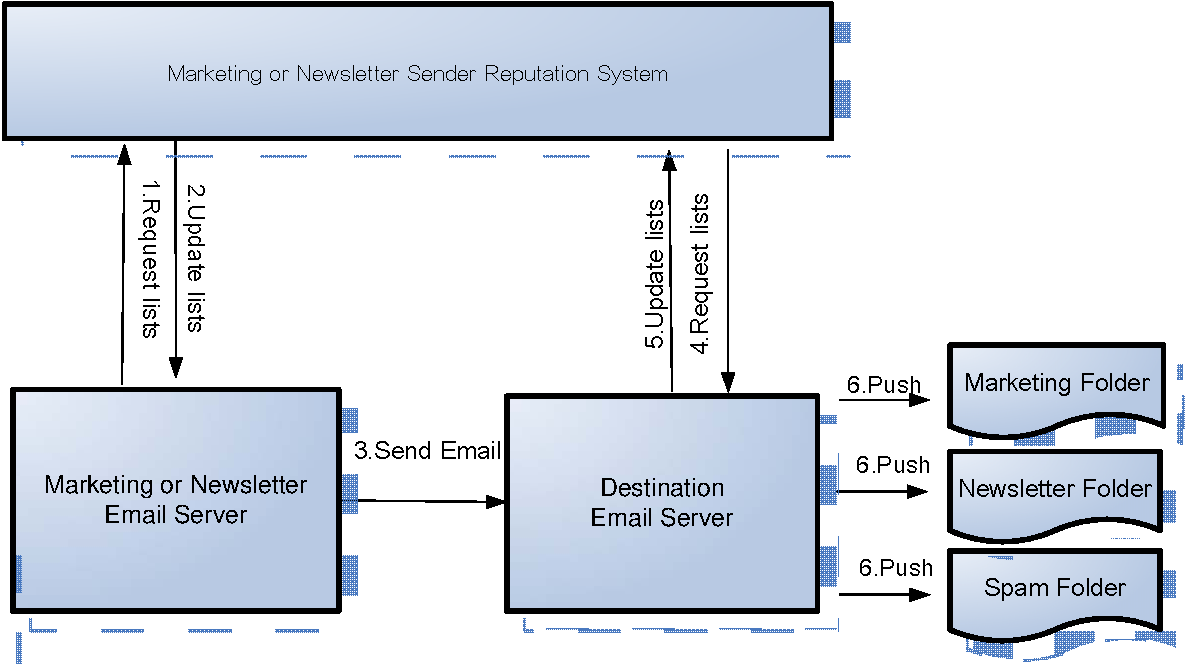
\includegraphics[width=0.48\textwidth]{1_FMNSRS.pdf}
\caption{Research design and process diagram.}
\label{fig:FMNRS}
\end{figure}

%\subsection{Method 1: The request from the recipient}
\subsection{The Request Method 1}
This method is used to help the recipients sending their marketing or newsletter email requests to the destination email server.
The request includes the email address of recipients and the marketing or newsletter email group wanted.
The request method 1 is
shown in Fig. \ref{fig:Method1} and described as follows:
%The request processes is as follows: 
1) The recipients submit their marketing or newsletter email groups wanted to the destination email server. 
% requests registered to The Destination Email Server what they want to receive the marketing or newsletter emails.
2) When the destination email server receives these requests from the recipients, it forward these requests to the Marketing or Newsletter Sender Reputation System (MNSRS) to register the wanted email with MNSRS. 
%2) If the Destination Email Server receives the registration of the recipients already, and then this request has been forwarded to the Marketing or Newsletter Sender Reputation System (MNSRS). The request includes the email address of recipients and type of content wanted.  
%The use of MNSRS to distribute these request to the Marketing or Newsletter Email Server that is a member already in the next step.
3) If the MNSRS receives such requests, it stores all requests of the recipients in the database itself and distributes each of the requests to the Marketing or Newsletter Email Servers by considering the matching of these requests.
For instance, the recipients want to receive movie email group that this request is sent to the Marketing or Newsletter Email Servers that provide information on the movie.
The marketing or newsletter email servers store the received requests in the database itself.
In this method, the marketing or newsletter email servers can send their information to the recipients efficiency that we explain in the sending marketing or newsletter email method.
%3) If the Marketing or Newsletter Email Servers receive the request of recipients, and then they store these request in their server to send their own emails to the recipients.

\begin{figure}
\centering
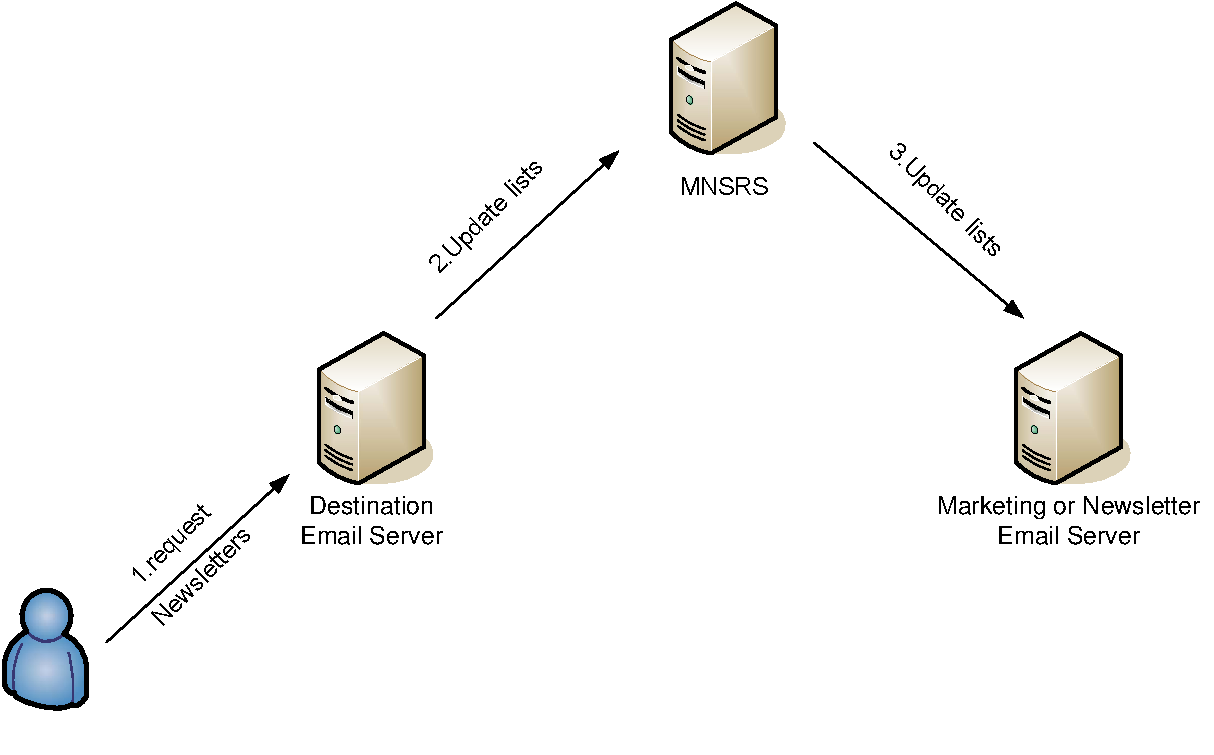
\includegraphics[width=0.48\textwidth]{2.pdf}
\caption{The processes of the request method 1.}
\label{fig:Method1}
\end{figure}

\subsection{The Request Method 2}
The recipients can request to receive the marketing or newsletter emails by subscription on the marketing or newsletter email servers.
The request method 2 is
shown in Fig. \ref{fig:Method2Process} and described as follows:
%The request method 2 is shown in Fig. \ref{fig:Method2Process}.
%The request process is as follows: 
%1) The recipients registered to the Destination Email Server what they want to receive the marketing or newsletter emails. 
1) The recipients can request to receive the emails by double opt-in \cite{Allman:DoubleOptIn} to subscribe of the marketing or newsletter email servers wanted.
%2) If the Destination Email Server receives the registration of the recipients already, and then this request has been forwarded to the Marketing or Newsletter Email Servers.
2) When the marketing or newsletter email servers receive the request and confirmation from the recipient, they send such request to MNSRS to update the list of recipients and the marketing or newsletter email group in a centralized database. 
3) Then MNSRS forward this request to the destination email server of recipients registered to update such data in a database of recipients. 

\begin{figure}
\centering
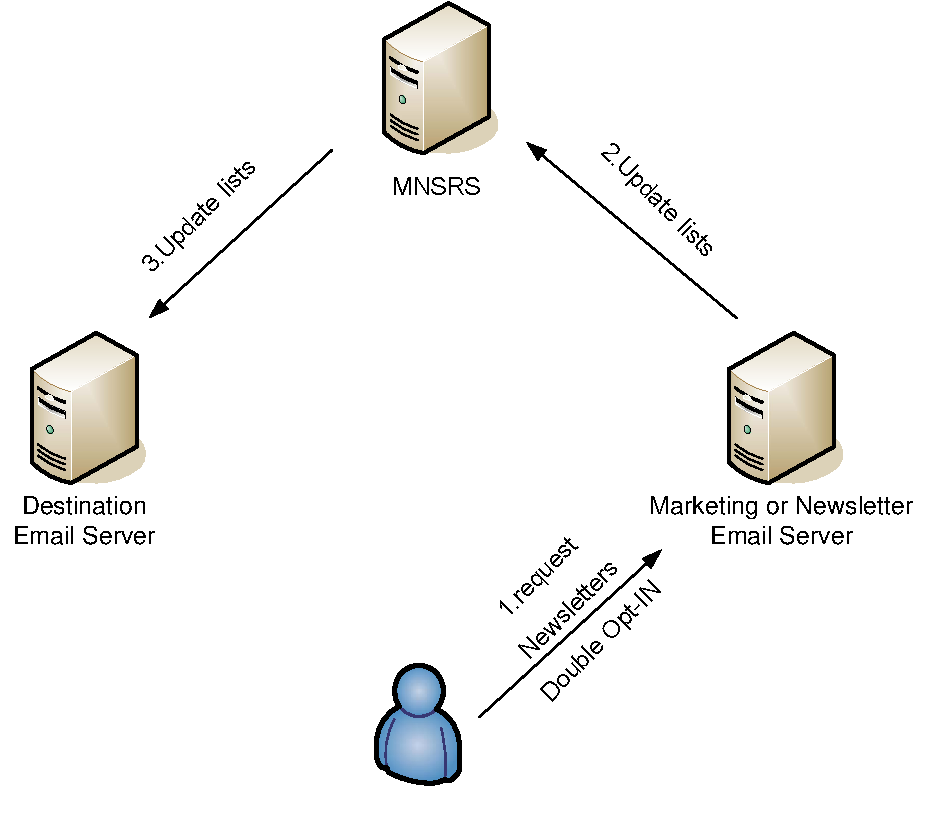
\includegraphics[width=0.45\textwidth]{3.pdf}
\caption{The processes of the request method 2.}
\label{fig:Method2Process}
\end{figure}

\subsection{The Sending Marketing or Newsletter Email Method}
\label{subsec:3}
The sending marketing or newsletter email method is
shown in Fig. \ref{fig:SendingMethod} and described as follows:
%The sending process is as follows: 
%1) The marketing or newsletter email servers connect to MNSRS to update the list and marketing or newsletter email group wanted of recipients.
1) The marketing or newsletter email server sends the marketing or newsletter emails to wanted recipient systems by considering the list and marketing or newsletter email group wanted of recipients in a database of sender.  
To update such datas in a database, there are two processes as follows: the marketing or newsletter email server can define a schedule to update automatically with MNSRS.
In addition, MNSRS can also define a schedule to send these datas to the marketing or newsletter email server for automatic updating. 
%1) The marketing or newsletter email servers connect to MNSRS to update the detail of recipients to match the MNSRS database.
%2) When the update is completed, the marketing or newsletter email servers send the marketing or newsletter emails to wanted recipients through the Destination Email Server of recipients.
2) When the destination email servers receive the marketing or newsletter emails, they classify and enter these emails into the inbox categories of wanted recipients in their domain such as Marketing, Newsletter and etc. 
If emails received are not to be desired, they are entered into the spam inbox.
%
In the classifying email group process, the destination email servers check
the list of senders, sender reputations, and wanted email groups each of the recipients in a database itself.
%
If such datas of the sender match datas in a database and the high reputation score sender, email is moved to the inbox categories of wanted recipients.
Otherwise, email is moved to the spam inbox.
% match the destination email server connect to MNSRS to update the list and marketing or newsletter email group wanted of recipients.
%If not match the destination email server enter this email into spam category.
A database of recipients is updated by MNSRS that both sides can define the schedule for automatic updating.

%3) The Destination Email Server connect to MNSRS to update the list of Marketing or Newsletter Mail Server and details of recipients under the destination domain only.
%4) The Destination Mail Server enter the email into the inbox categories of wanted recipients as Marketing, Newsletter or Spam in their domain.

\begin{figure}
\centering
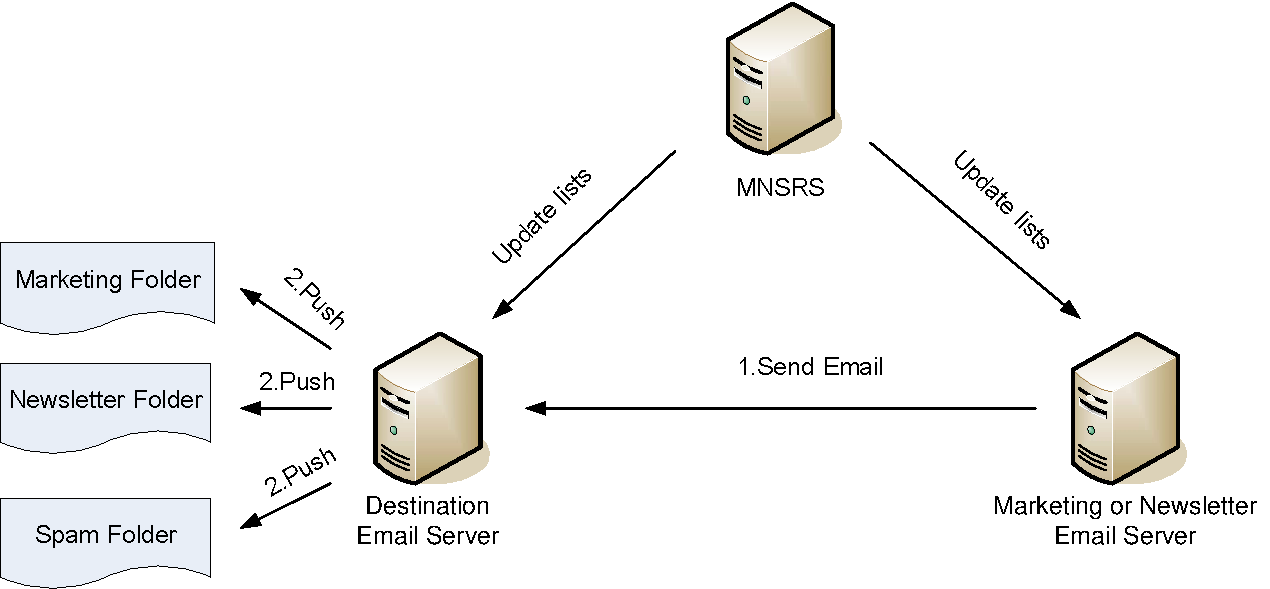
\includegraphics[width=0.48\textwidth]{4.pdf}
\caption{The sending marketing or newsletter email method.} 
\label{fig:SendingMethod}
\end{figure}

\subsection{The False Reporting Method}
The false reporting method is
shown in Fig. \ref{fig:FaultReportingMethod} and described as follows:
%1) Marketing or Newsletter Email Server send the marketing or newsletter emails to the recipients registered through the Destination Email Server of recipients.
%2) Destination Email Server enters the email to mail box categories of the recipients using the wanted data of recipients from the MNSRS.
1) When the recipients receive the unwanted marketing or newsletter emails and these emails are not in the spam inbox, the recipients can move these emails to spam inbox to report back to the senders.
2) Then the destination email servers of recipients reported connect to the MNSRS to unsubscribe the marketing or newsletter email servers wanted.
%
Besides that, the MNSRS calculates new reputation score each of the senders canceled by using the statistics reports.
%to prepare the sender Reputation of Marketing or Newsletter Email Server from such the statistics reported.
3) The MNSRS send the lists of unwanted recipients to the marketing or newsletter email servers that send email to unwanted recipients for updating recipient database. 

\begin{figure}
\centering
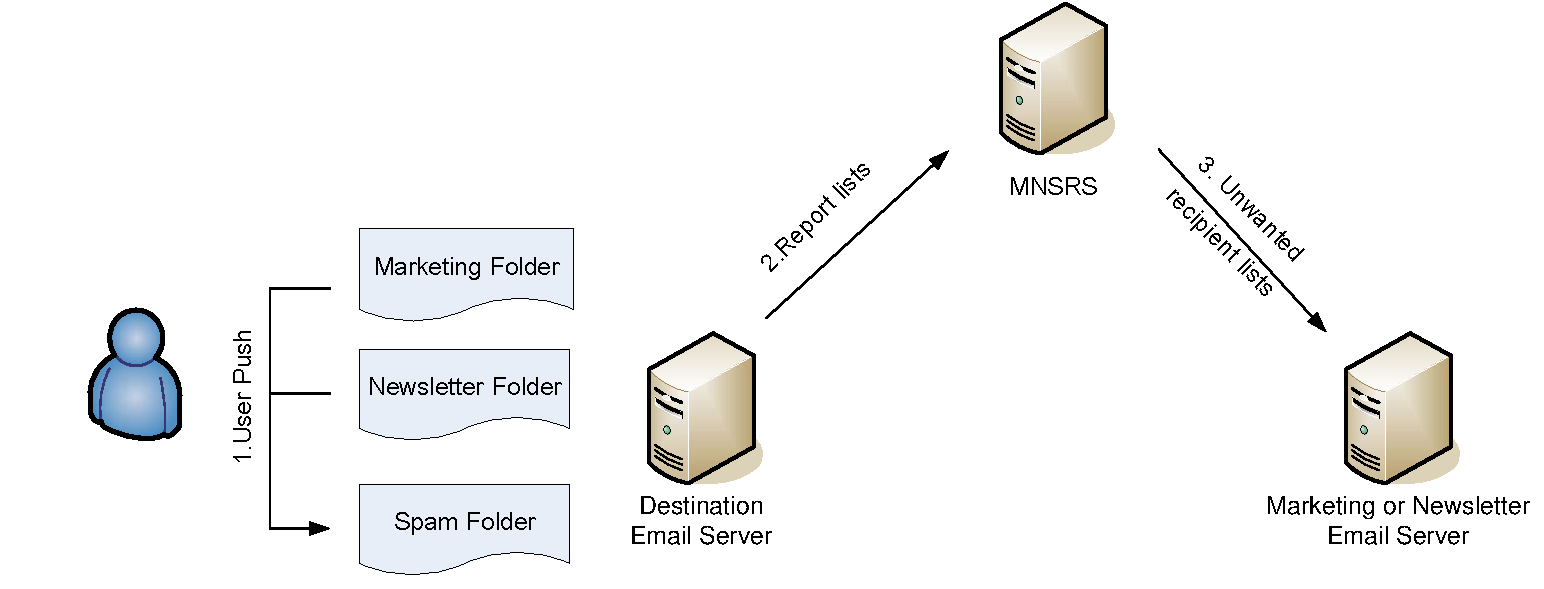
\includegraphics[width=0.48\textwidth]{5.pdf}
\caption{The false reporting method.}
\label{fig:FaultReportingMethod}
\end{figure}

\subsection{The Sender Reputation Method}
The sender reputation method by using MNSRS is
shown in Fig. \ref{fig:ReputationMethod} and described as follows:
1) While the recipients move the unwanted marketing or newsletter emails to spam inbox, the destination email servers of recipients reported will receive the these false reports
%2) Then the recipients report to Destination Email Server that they receive the list of unwanted emails.
2) Such the destination email server connect to the MNSRS to unsubscribe the marketing or newsletter email servers wanted.
The MNSRS updates own recipient database and calculates new reputation score each of the senders canceled based on the centralized recipient feedback by using this formula:
% to prepare the sender Reputation of Marketing or Newsletter Email Server from such the statistics reported.
%The sender reputation can be calculated by using this formula:\\

$$ \text{reputation} =  \frac{ 100\times{\text{(asm - aur)}}}{\text{asm}} $$
where\mbox{ }\\
%asm = all of the sending marketing emails.\mbox{ }\\
asm = Total of the sending marketing or newsletter emails each of the senders.\\
aur = Total of spam  marketing or newsletter emails that reported by the unwanted recipients.


\begin{figure}
\centering
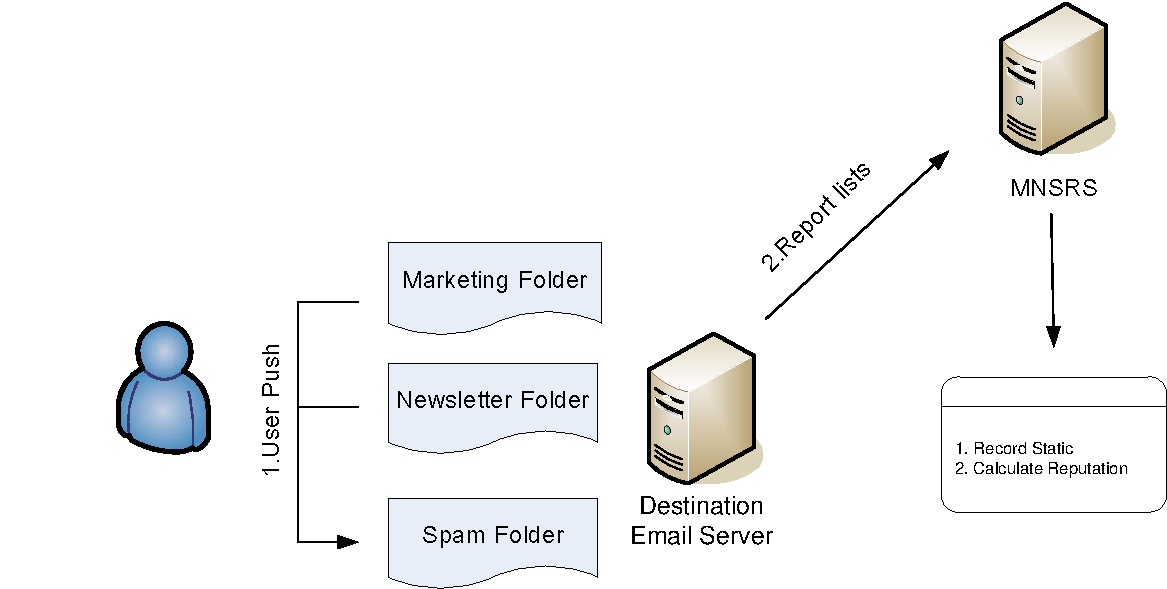
\includegraphics[width=0.48\textwidth]{6.pdf}
\caption{The sender reputation method by using MNSRS.}
\label{fig:ReputationMethod}
\end{figure}

\subsection{The Sender and Recipient Authentication Method}
In the sending and receiving marketing or newsletter emails process between the marketing or newsletter email servers and the destination email servers, SPF \cite{wong,NguyenTuanAnh,Seike} is used to confirmed both good email systems.
%The Marketing or Newsletter Email Server and the Destination Email Server update the list of the recipients received the wanted marketing or newsletter email.
%Then they send these email to the recipients to meet the demand.
The conditions for sending and receiving email are as follows:
The registered email systems of the senders and the recipients must support SPF method to send and receive emails.
The process diagram is shown in Fig. \ref{fig:AuthenticationMethod}.

\begin{figure}
\centering
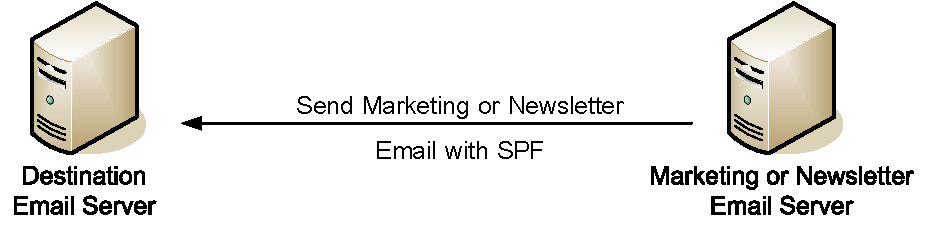
\includegraphics[width=0.48\textwidth]{7.pdf}
\caption{The sender and recipient authentication method.}
\label{fig:AuthenticationMethod}
\end{figure}


\section{Experimental Results}
According to the author has designed and tested the FMNSRS system that can classify the marketing or newsletter email group matching the real needs of the recipients better than the traditional email system.
It works well especially when the emails with the
contents in the local language is not in English.
In addition to that, all processes of the FMNSRS system are run automation.
The administrators do not need to modify the database itself. 
The users of FMNSRS system also feel no difference from using the general email systems. 
Moreover, this paper is also able to identify the senders as either quality or not quality.
The experimental samples for this research are shown in Table \ref{table_inputData} and Table \ref{table_emailDataset_checkRecord} shows the email data set and checking record.

\begin{table}[!t]
\renewcommand{\arraystretch}{1.2}
\caption{Summary of the experimental samples}
\label{table_inputData}
\centering
\begin{tabular}{c|c}
\hline
\bfseries The Experimental Sample & \bfseries Summary\\
\hline
Number of the general email systems & 10\\
\hline
Number of the marketing or newsletter email systems & 10\\
\hline
Number of the email accounts & 40\\
\hline
Number of the normal emails & 1000\\
\hline
Number of the marketing or newsletter emails& 1000\\
\hline
Number of the spam emails& 1000\\
\hline
\end{tabular}
\end{table}

\begin{table}[!t]
\renewcommand{\arraystretch}{1.2}
\caption{Email Data Set and Checking Record}
\label{table_emailDataset_checkRecord}
\centering
\begin{tabular}{c|c}
\hline
\bfseries Email Data Set & \bfseries Checking Record\\
\hline
Email of the sender & Email records of the marketing or newsletter sender\\
\hline
Email of the recipient & Email records of the marketing or newsletter recipient\\
\hline
IP address of the sender & IP address of the sender match the DNS reliability\\
\hline
content (keyword) & content filter (keyword)\\ 
\hline
- & sender reputation (score1,check-push) \\
\hline
- & sender reputation (score2,check-push) \\
\hline
- & sender reputation (score3,check-push) \\
\hline
- & sender reputation (score4,check-push) \\
\hline
- & DNSBL by IP address \\
\hline
- & DNSWL by IP address\\
\hline
\end{tabular}
\end{table}

To analyze system performance for this paper, there are two methods for analysis described in the following subsections.

\subsection{True positive (TP)}
This method is used to analyze the accuracy of the detection email which can be calculated by using this formula:\\
$$ \text{NEAR} =  \frac{\text{NofNEDetectedNE}}{\text{NofNEDetectedNE + NofNEDetectedFault}} \times 100 $$\\
$$ \text{MEAR} =  \frac{\text{NofMEDetectedME}}{\text{NofMEDetectedME + NofMEDetectedFault}} \times 100 $$\\
$$ \text{SEAR} =  \frac{\text{NofSEDetectedSE}}{\text{NofSEDetectedSE + NofSEDetectedFault}} \times 100 $$\\

%put these in Notation table
\begin{table}[!t]
\renewcommand{\arraystretch}{1.2}
\caption{Variable Description for TP}
\label{table_variableTP}
\centering
\begin{tabular}{c|l}
\hline
\bfseries Variables & \multicolumn{1}{c}{\bfseries Description}\\
\hline
NEAR & The accurate rate of the normal email detection.\\
\hline
NofNEDetectedNE & The number of the normal email that are detected as \\ & the normal email.\\
\hline
NofNEDetectedFault & The number of the normal emails detected fault.\\
\hline
MEAR & The accurate rate of the marketing or newsletter email \\ & detection.\\
\hline
NofMEDetectedME & The number of the marketing or newsletter email that are \\ & detected as the marketing or newsletter email.\\
\hline
NofMEDetectedFault & The number of the marketing or newsletter email detected \\ & fault.\\
\hline
SEAR & The accurate rate of the spam email detection.\\
\hline
NofSEDetectedSE & The number of the spam email that are detected as\\ & the spam email.\\
\hline
NofSEDetectedFault & The number of the spam email detected fault.\\
\hline
\end{tabular}
\end{table}

Table \ref{table_variableTP} summarizes the notation for The TP Analysis.
Fig. \ref{fig:resultTP} and Table \ref{table_resultsTP} show the results of the TP
analysis.
As a
results, this novel process can detect the normal emails accurately 81.90\% and 45.26\% more than the traditional process.
Furthermore, the novel process can detect the marketing or newsletter email accurately 73.30\% and the spam email accurately 62.44\%.
These results are an acceptable accurate
rate.

\begin{figure}
\centering
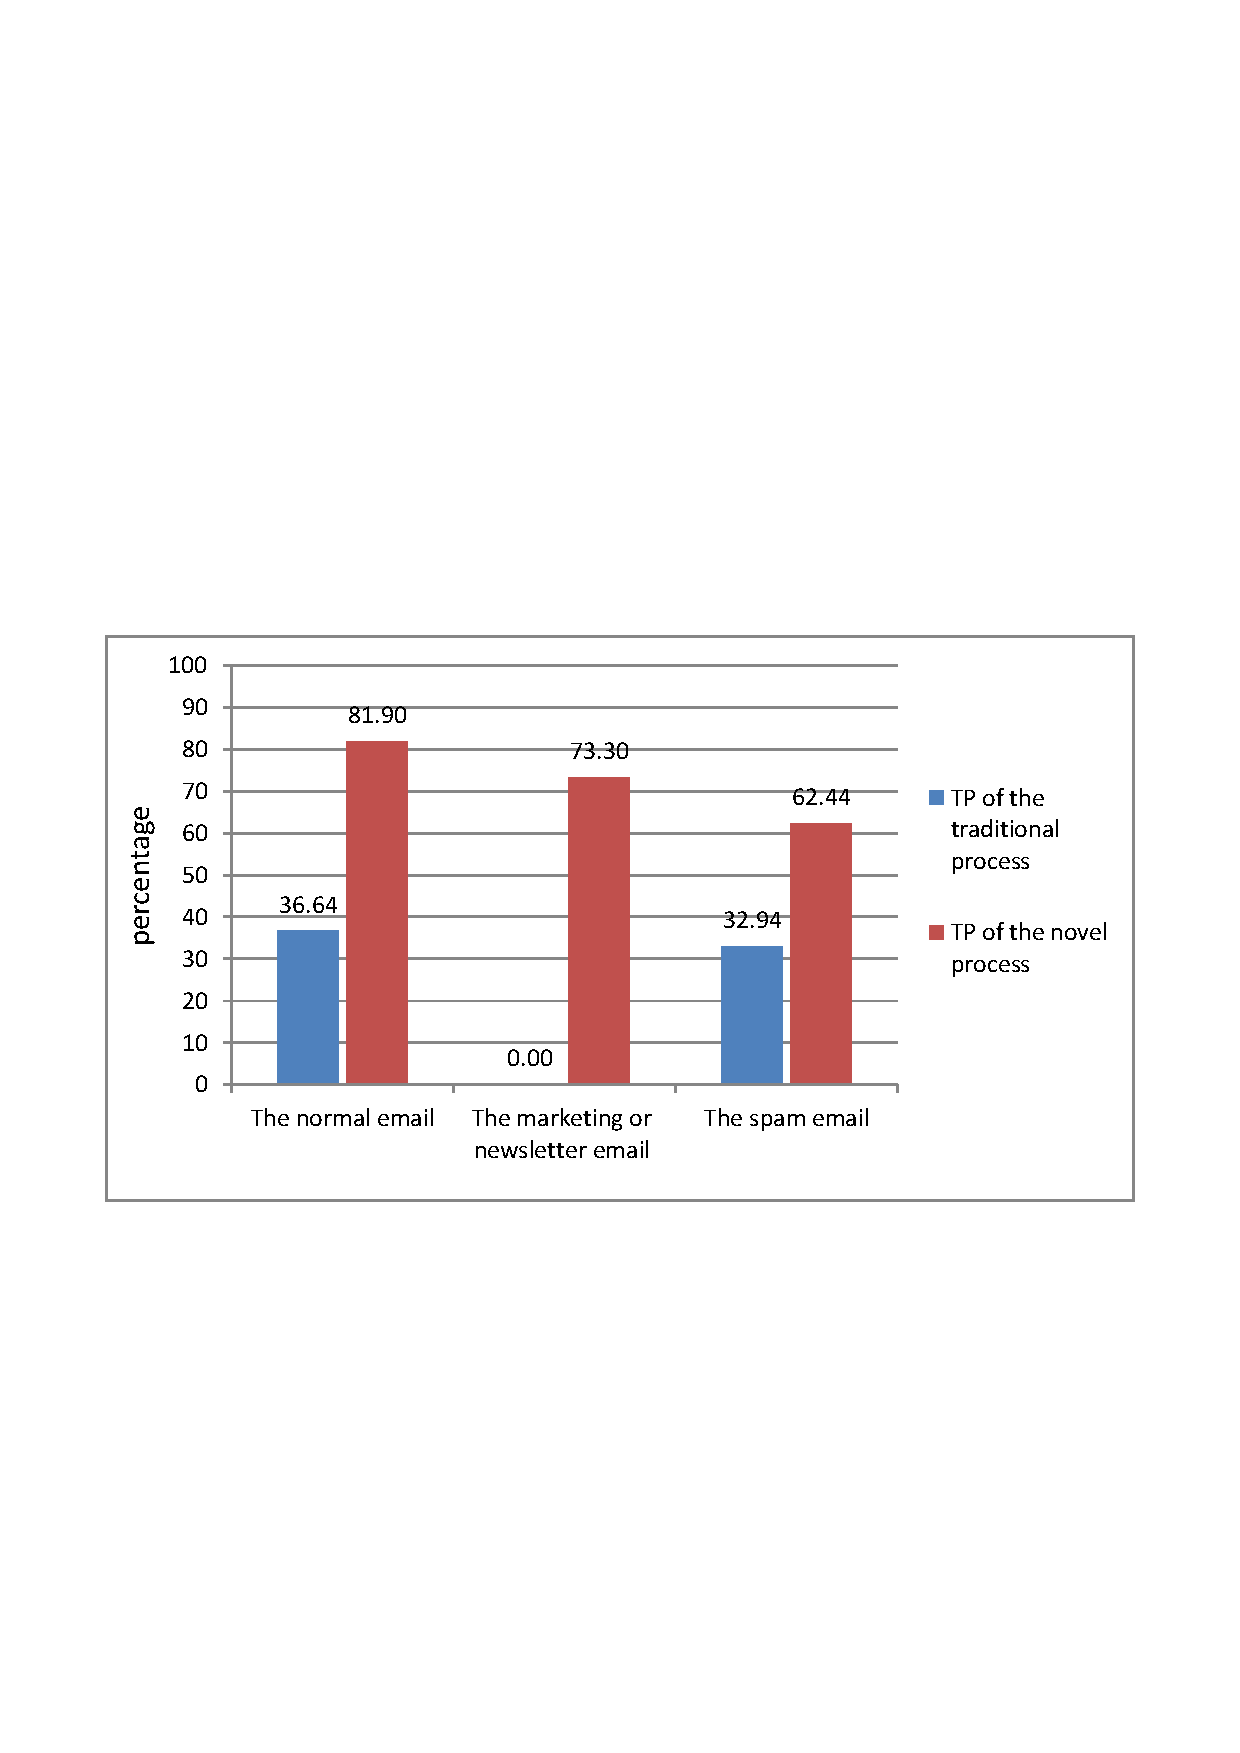
\includegraphics[width=0.48\textwidth]{8.pdf}
\caption{The results of the true positive analysis.}
\label{fig:resultTP}
\end{figure}

\begin{table}[!t]
\renewcommand{\arraystretch}{1.2}
\caption{The Results of The True Positive Analysis}
\label{table_resultsTP}
\centering
\begin{tabular}{c|c|c}
\hline
\bfseries Accurate Rate & \bfseries Traditional process & \bfseries Novel process\\
\hline
The normal email & 36.64\% & 81.90\%\\
\hline
The marketing or newsletter email & 0.00\% & 73.30\%\\
\hline
The spam email & 32.94\% & 62.44\%\\
\hline
\end{tabular}
\end{table}

%FP analysis
\subsection{False positive (FP)}
This method is used to analyze email fault detection which can be calculated by using this formula:\\
$$ \text{NEFR} =  \frac{\text{NofNEDetectedFault}}{\text{NofNEDetectedNE + NofNEDetectedFault}} \times 100 $$\\
$$ \text{MEFR} =  \frac{\text{NofMEDetectedFault}}{\text{NofMEDetectedME + NofMEDetectedFault}} \times 100 $$\\
$$ \text{SEFR} =  \frac{\text{NofSEDetectedFault}}{\text{NofSEDetectedSE + NofSEDetectedFault}} \times 100 $$\\

%put these in Notation table
\begin{table}[!t]
\renewcommand{\arraystretch}{1.2}
\caption{Variable Description for FP}
\label{table_variableFP}
\centering
\begin{tabular}{c|l}
\hline
\bfseries Variables & \multicolumn{1}{c}{\bfseries Description}\\
\hline
NEFR & The fault rate of the normal email detection.\\
\hline
MEFR & The fault rate of the marketing or newsletter email detection.\\
\hline
SEFR & The fault rate of the spam email detection.\\
\hline
\end{tabular}
\end{table}

Table \ref{table_variableFP} summarizes the notation for The FP Analysis.
Fig. \ref{fig:resultFP} and Table \ref{table_resultsFP} show the results of the FP
analysis.
As a
results, this novel process can detect the normal emails wrongly 18.10\% and 45.26\% more efficient than the traditional process.
Moreover, the novel process can detect the marketing or newsletter email wrongly 26.70\% and the spam email wrongly 37.56\%. 

\begin{figure}
\centering
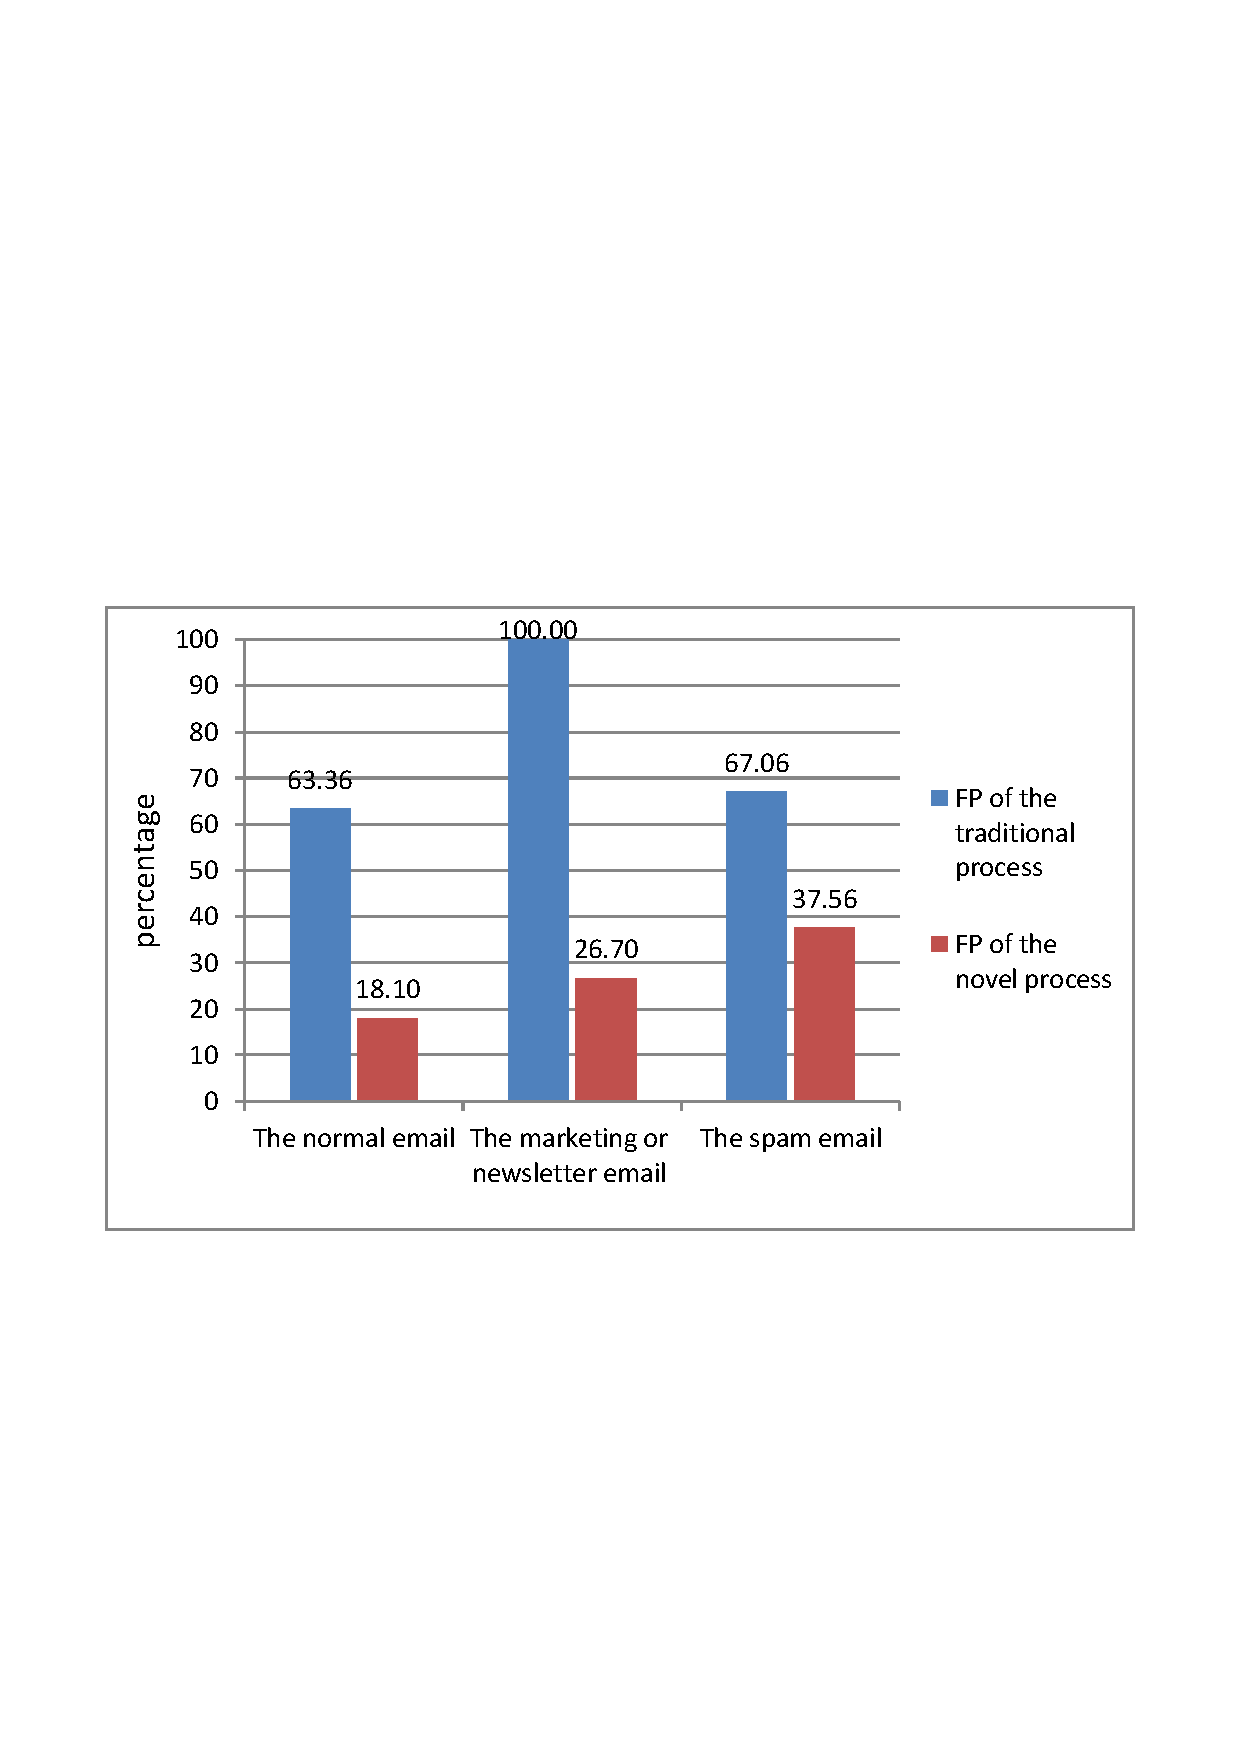
\includegraphics[width=0.48\textwidth]{9.pdf}
\caption{The results of the false positive analysis.}
\label{fig:resultFP}
\end{figure}

\begin{table}[!t]
\renewcommand{\arraystretch}{1.2}
\caption{The Results of The False Positive Analysis}
\label{table_resultsFP}
\centering
\begin{tabular}{c|c|c}
\hline
\bfseries Fault Rate & \bfseries Traditional process & \bfseries Novel process\\
\hline
The normal email & 63.36\% & 18.10\%\\
\hline
The marketing or newsletter email & 100.00\% & 26.70\%\\
\hline
The spam email & 67.06\% & 37.56\%\\
\hline
\end{tabular}
\end{table}

\section{Conclusion and Future Directions}
The testing results from the previous section show that this technique can improve the detection capability of the email detection process.
The novel system can classify the type of email, marketing or newsletter, matching the real needs of the recipient better than the traditional system.
In addition, it can help facilitate email management for administrators.
However, there is also disadvantages as follows. 
1) If the amount of the registration or the statistic are not enough,  this system can detect the emails accuracy decreases.
2) This technique is necessary to use the request and response data exchange several times.
In the future work, we intend to improve the exchange process less complicated.
In addition to that, we intend to improve the detection accuracy although there is not enough information.




% conference papers do not normally have an appendix


% use section* for acknowledgement
\section*{Acknowledgment}
This work was supported by Mahanakorn University of Technology and the Defence Technology Institute (Public Organization), Thailand.





% trigger a \newpage just before the given reference
% number - used to balance the columns on the last page
% adjust value as needed - may need to be readjusted if
% the document is modified later
%\IEEEtriggeratref{8}
% The "triggered" command can be changed if desired:
%\IEEEtriggercmd{\enlargethispage{-5in}}

% references section

% can use a bibliography generated by BibTeX as a .bbl file
% BibTeX documentation can be easily obtained at:
% http://www.ctan.org/tex-archive/biblio/bibtex/contrib/doc/
% The IEEEtran BibTeX style support page is at:
% http://www.michaelshell.org/tex/ieeetran/bibtex/
%\bibliographystyle{IEEEtran}
% argument is your BibTeX string definitions and bibliography database(s)
%\bibliography{IEEEabrv,../bib/paper}
%
% <OR> manually copy in the resultant .bbl file
% set second argument of \begin to the number of references
% (used to reserve space for the reference number labels box)

\bibliographystyle{IEEEtran}
\IEEEtriggeratref{12}
\bibliography{IEEEabrv,bibRef}

%\begin{thebibliography}{1}

%\bibitem{IEEEhowto:kopka}
%H.~Kopka and P.~W. Daly, \emph{A Guide to \LaTeX}, 3rd~ed.\hskip 1em plus
%  0.5em minus 0.4em\relax Harlow, England: Addison-Wesley, 1999.

\ %end{thebibliography}




% that's all folks
\end{document}


